% !TeX spellcheck = en_GB
% !TeX encoding = UTF-8
% !TeX root = sikdd2026.tex
% !TeX TS-program = pdflatex
% !BIB TS-program = biber
%%
%% "Category, Not Severity" -- SiKDD 2026, Information Society multiconference.
%% HARD LIMIT: 4 pages including references. Check the page count on every compile.
%%
\documentclass[sigconf,natbib=false, language=english]{acmart}

\usepackage[datamodel=acmdatamodel, style=acmnumeric, backend=biber]{biblatex}
\addbibresource{refs.bib}
% References compressed to hold the venue's 4-page limit, which includes them.
\ExecuteBibliographyOptions{maxbibnames=3, minbibnames=1}
\renewcommand*{\bibfont}{\fontsize{6.0}{6.7}\selectfont}
\usepackage{tikz}
\usetikzlibrary{positioning, arrows.meta}
\definecolor{inkc}{HTML}{1F2A37}
\definecolor{accentc}{HTML}{8C2F39}
\definecolor{halfc}{HTML}{B0564A}
\definecolor{bluec}{HTML}{3D5A80}
\definecolor{grayc}{HTML}{5C6670}

\AtBeginDocument{%
  \providecommand\BibTeX{{%
    Bib\TeX}}}

\setcopyright{rightsretained}
\copyrightyear{2026}
\acmDOI{}
\acmConference[Information Society 2026]{Information Society 2026: 29th international multiconference}{5--9 October 2026}{Ljubljana, Slovenia}
\acmISBN{}
\settopmatter{printccs=false, printacmref=false}
\geometry{a4paper}
\raggedbottom  % avoid stretched gaps above headings on the last page

\begin{document}

\title[Category, Not Severity]{Category, Not Severity: How Large Language Models
  Misclassify AI Incidents Under the EU AI Act Risk Taxonomy}

\author{Stefan Kofilovski}
\email{stefan.kofilovski@gmail.com}
\affiliation{%
  \institution{Ss. Cyril and Methodius University}
  \city{Skopje}
  \country{North Macedonia}
}

\author{Georgi Trajkov}
\email{geotrajkov0@gmail.com}
\affiliation{%
  \institution{Jožef Stefan Institute}
  \institution{Jožef Stefan International Postgraduate School}
  \city{Ljubljana}
  \country{Slovenia}}

\begin{abstract}
The EU AI Act assigns risk categories by what an AI system does and where it is
deployed, not by how much harm it has caused. Incident trackers increasingly assign
these categories with large language models (LLMs), yet a recent audit found several
frontier LLMs scoring below chance on the Act's category while doing well on other
taxonomies. To test whether the failure is procedural, a lawyer labelled 144 incidents
from the AI Incident Database against a published rubric derived from the Act, and 14
LLMs classified them under a basic prompt and under a step-by-step prompt that walks
the Act's rules in order. Agreement with the expert ranges from $\kappa = -0.07$ to
$0.65$ under the basic prompt and from $0.30$ to $0.70$ under the step-by-step prompt
(means 0.42 and 0.50). We show that the errors are directional: LLMs over-classify
incidents outside Annex III and stay unbiased inside it, as expected if they judge
severity rather than category. Spelling the rules out roughly halves that outward
bias, at the cost of a smaller opposite one inside Annex III. For automated
monitoring, categories assigned outside Annex III are the first place to spend human
review. Rubric, prompts and labels are released.
\end{abstract}

\keywords{EU AI Act, risk classification, large language models, AI incidents,
  regulatory compliance, AI governance}

\maketitle

\section{Introduction}

\begin{figure}[t]
  \centering
  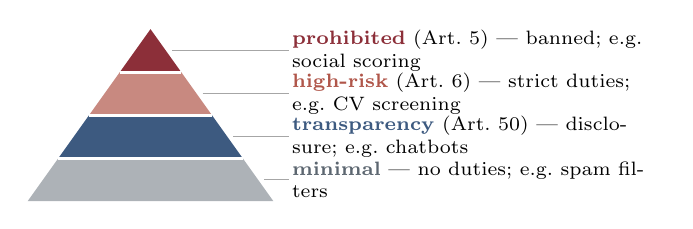
\begin{tikzpicture}[font=\scriptsize, scale=0.78]
    % pyramid: apex y=2.8, base half-width 2.0 (drawn at 0.78 scale)
    \fill[grayc!50]  (-2.0,0)    -- (2.0,0)    -- (1.5,0.7)  -- (-1.5,0.7)  -- cycle;
    \fill[bluec]     (-1.5,0.7)  -- (1.5,0.7)  -- (1.0,1.4)  -- (-1.0,1.4)  -- cycle;
    \fill[halfc!70]  (-1.0,1.4)  -- (1.0,1.4)  -- (0.5,2.1)  -- (-0.5,2.1)  -- cycle;
    \fill[accentc]   (-0.5,2.1)  -- (0.5,2.1)  -- (0,2.8)              -- cycle;
    \foreach \y in {0.7,1.4,2.1} \draw[white, line width=1.1pt]
      ({-2.0*(1-\y/2.8)},\y) -- ({2.0*(1-\y/2.8)},\y);
    \foreach \y/\xa in {2.45/0.35, 1.75/0.85, 1.05/1.35, 0.35/1.85}
      \draw[black!35, thin] (\xa,\y) -- (2.25,\y);
    \node[anchor=west, text width=4.7cm, align=left, inner sep=1pt] at (2.25,2.45)
      {\textcolor{accentc}{\textbf{prohibited}} (Art.~5) --- banned; e.g.\ social scoring};
    \node[anchor=west, text width=4.7cm, align=left, inner sep=1pt] at (2.25,1.75)
      {\textcolor{halfc}{\textbf{high-risk}} (Art.~6) --- strict duties; e.g.\ CV screening};
    \node[anchor=west, text width=4.7cm, align=left, inner sep=1pt] at (2.25,1.05)
      {\textcolor{bluec}{\textbf{transparency}} (Art.~50) --- disclosure; e.g.\ chatbots};
    \node[anchor=west, text width=4.7cm, align=left, inner sep=1pt] at (2.25,0.35)
      {\textcolor{grayc}{\textbf{minimal}} --- no duties; e.g.\ spam filters};
  \end{tikzpicture}
  \caption{The four risk categories of the EU AI Act, with typical systems. How severe
  an incident's real-world outcome was plays no part in the assignment.}
  \label{fig:tiers}
\end{figure}

AI incident databases have become policy infrastructure. The AI Incident Database
(AIID) collects public reports of cases in which a deployed AI system caused or nearly
caused harm (\textbf{incidents}), each stored as a short structured record linked to
the underlying news coverage~\cite{mcgregor2021}. Trackers built on top of it, such as
the MIT AI Incident Tracker~\cite{mit_tracker_2026}, attach classification schemes
(\textbf{taxonomies}) to every incident, and downstream readers rely on the resulting
labels. One of those taxonomies is the risk category of the EU AI
Act~\cite{aiact2024} --- hereafter the Act; ``Art.~6(3)'' means paragraph~3 of its
Article~6 --- which sorts AI systems into four categories: \emph{prohibited}, \emph{high-risk}, \emph{transparency} and
\emph{minimal}, as seen in Figure~\ref{fig:tiers}. Annotating thousands of records by
hand is infeasible, so these labels are increasingly produced by large language models
(\textbf{LLMs}).

This shortcut has a documented weak spot. In June 2026 the MIT AI Risk Initiative
audited its own tracker against two human reviewers and reported that four of eight
frontier LLMs scored a \emph{negative} quadratic weighted kappa --- worse than chance
--- on the AI Act category while clearing the human baseline on other
taxonomies~\cite{mit_tracker_2026}. The audit rested on ten incidents, on which the
prompt refinements that repaired the score were also developed --- a limitation the
authors state while calling for held-out data.

We take up that invitation and add a hypothesis about \emph{why} the failure occurs.
The Act's classification logic is categorical and function-based. A system is
high-risk because it is a safety component of a product
that already undergoes third-party safety certification, such as machinery or a
medical device (Art.~6(1), \textbf{Annex~I}), or because it is used in one of eight
sensitive application areas --- among them employment, education, credit and law
enforcement (Art.~6(2), \textbf{Annex~III}) --- subject to a narrow exception for
purely preparatory or procedural roles (Art.~6(3)), unavailable where the system
profiles people. How severe the real-world consequences of an incident were is not a
factor in this classification.

We hypothesise that LLMs nevertheless tend to classify incidents by the severity of
the outcome --- the question a short record lets them answer --- rather than by the
category question the statute asks. We call this \textbf{severity substitution}. If
it occurs, the errors should be systematic rather than random: over-classification of
severe-sounding incidents outside Annex~III, and under-classification of
mundane-sounding incidents inside it.

Our contributions are (i) a lawyer-written, published annotation rubric that turns
the Act's classification rules into a procedure for short incident records; (ii) an
expert-labelled sample of 144 AIID incidents, fourteen times the size of the audit
above; (iii) a 14-LLM comparison under a basic and a step-by-step prompt; and (iv) an
error analysis by Annex~III membership that locates where severity substitution
occurs.

\section{Related Work}

\textbf{Annotating AI incidents.} The AIID was built to make AI incidents citable
and comparable~\cite{mcgregor2021}, and the taxonomies attached to its records now
feed risk repositories and policy reporting~\cite{slattery2026}. Most such taxonomies
describe what happened: the MIT AI Risk Repository's domain taxonomy, which the
tracker of Section~1 applies alongside the Act's category, sorts a record into one of
seven domains such as discrimination, privacy or misinformation~\cite{slattery2026}.
The Act's category is different in kind: it asks what the system is for, not what it
did. Paeth et al.~\cite{paeth2025} review more than 750 incident records under two
descriptive taxonomies and find that uncertainty about cause, extent of harm and
technical detail is unavoidable in incident reporting. That caps how far any two
annotators --- human or machine --- can agree, and makes ``the record does not say''
a substantive answer rather than a failure.

\textbf{Automating AI Act classification.} The closest prior work is
CORTEX~\cite{cortex2025}, a taxonomy of 29 technical vulnerability groups applied to
over 1,200 AIID incidents, each mapped onto the AI Act and related frameworks and
given a composite \emph{risk score} that is explicitly severity- and
exposure-weighted, not validated against legal judgements of the Act's own
categories. Our question is the complement of theirs: not how risky a system is, but
which category the statute assigns it to, a question in which severity plays no part.

\textbf{The difficulty of the classification.} Leinarte~\cite{leinarte2024} shows how
much interpretive work the high-risk rules (Art.~6 and Annex~III, Section~3) demand
in practice. Empirically, experts applying a pre-final draft of the Act could not
clearly classify roughly 40\% of 106 real corporate AI systems~\cite{appliedai}, and
the MIT audit reports a human--human agreement of only $\kappa = 0.56$ on AI Act
categories~\cite{mit_tracker_2026}. The task is genuinely hard for people, which is
why we frame results as expert--model disagreement rather than model accuracy. A
structured, question-by-question assessment has been proposed for related governance
judgements~\cite{constantinides2024}; our step-by-step prompt tests whether the same
structure helps LLMs with the Act.

\section{The Classification Rules and the Annotation Rubric}

\begin{figure}[t]
  \centering
  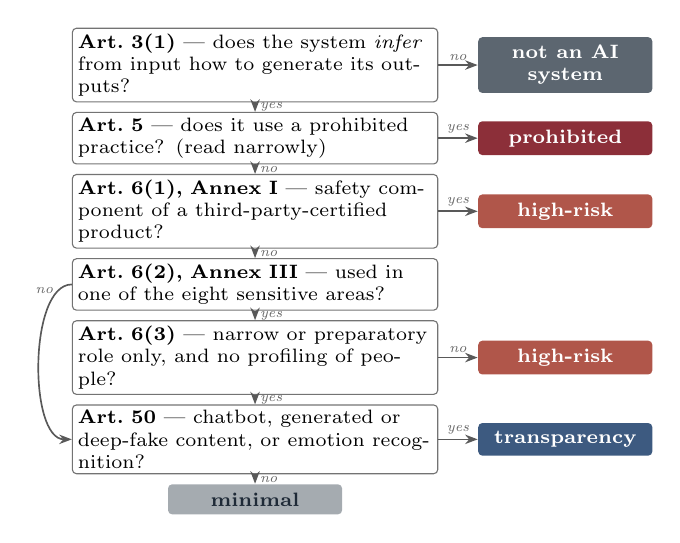
\begin{tikzpicture}[
      font=\scriptsize,
      q/.style={draw=black!55, rounded corners=1.5pt, align=left, text width=4.5cm,
                inner sep=2pt},
      t/.style={rounded corners=1.5pt, align=center, text width=2.0cm, inner sep=3pt,
                text=white, font=\scriptsize\bfseries},
      e/.style={font=\tiny\itshape, inner sep=1.5pt, black!60},
      arr/.style={-{Stealth[length=1.6mm]}, black!65, semithick},
      node distance=1.2mm and 5mm]
    \node[q] (q1) {\textbf{Art.~3(1)} --- does the system \emph{infer} from input how
      to generate its outputs?};
    \node[q, below=of q1] (q2) {\textbf{Art.~5} --- does it use a prohibited practice?
      (read narrowly)};
    \node[q, below=of q2] (q3) {\textbf{Art.~6(1), Annex~I} --- safety component of a
      third-party-certified product?};
    \node[q, below=of q3] (q4) {\textbf{Art.~6(2), Annex~III} --- used in one of the
      eight sensitive areas?};
    \node[q, below=of q4] (q5) {\textbf{Art.~6(3)} --- narrow or preparatory role
      only, and no profiling of people?};
    \node[q, below=of q5] (q6) {\textbf{Art.~50} --- chatbot, generated or deep-fake
      content, or emotion recognition?};
    \node[t, fill=grayc,   right=of q1] (tnot)  {not an AI system};
    \node[t, fill=accentc, right=of q2] (tproh) {prohibited};
    \node[t, fill=halfc,   right=of q3] (thigh1){high-risk};
    \node[t, fill=halfc,   right=of q5] (thigh2){high-risk};
    \node[t, fill=bluec,   right=of q6] (ttra)  {transparency};
    \node[t, fill=grayc!55, text=inkc, below=of q6] (tmin) {minimal};
    \draw[arr] (q1) -- node[e, above] {no}  (tnot);
    \draw[arr] (q2) -- node[e, above] {yes} (tproh);
    \draw[arr] (q3) -- node[e, above] {yes} (thigh1);
    \draw[arr] (q5) -- node[e, above] {no}  (thigh2);
    \draw[arr] (q6) -- node[e, above] {yes} (ttra);
    \draw[arr] (q1) -- node[e, right] {yes} (q2);
    \draw[arr] (q2) -- node[e, right] {no}  (q3);
    \draw[arr] (q3) -- node[e, right] {no}  (q4);
    \draw[arr] (q4) -- node[e, right] {yes} (q5);
    \draw[arr] (q5) -- node[e, right] {yes} (q6);
    \draw[arr] (q6) -- node[e, right] {no}  (tmin);
    \draw[arr] (q4.west) .. controls +(-0.55,0) and +(-0.55,0) .. (q6.west)
      node[e, pos=0.12, left] {no};
  \end{tikzpicture}
  \caption{The classification procedure that the rubric encodes and the step-by-step
  prompt follows. Art.~50 duties are recorded even where a higher category already
  applies.}
  \label{fig:test}
\end{figure}

The rubric answers a hypothetical question: if the system involved in this incident
were placed on the EU market today, which risk category would it fall under? The Act is
assumed to apply --- most incidents predate it or occurred outside the EU --- and the
object of classification is the system and its intended purpose, not the harm in the
record. Figure~\ref{fig:test} sketches the procedure; below, how each step is read on
incident records.

\textbf{Is it an AI system at all?} A purely deterministic, rule-based process is not
an AI system under Art.~3(1) and is recorded as such; the definition is broad, so this
disposes of few incidents.

\textbf{Does it use a prohibited practice?} The eight prohibited practices of Art.~5
--- social scoring and untargeted scraping of facial images among them; not to be
confused with the eight sensitive areas of Annex~III --- are read narrowly, as
prohibitions must be. Under Art.~5(1)(a), a subliminal or purposefully
manipulative technique must materially distort behaviour by \emph{appreciably}
impairing informed decision-making and thereby cause, or be likely to cause,
\emph{significant} harm. Intent to harm is not required, but the technique must be
attributable to how the system was trained or configured; ordinary hallucination does
not qualify. A third party who misuses a general-purpose
generator to run a fraud is therefore a \emph{user} of a tool, not the provider of a
prohibited system --- such incidents fall under Art.~50 instead; a system
\emph{configured} for the deceptive purpose remains prohibited.

\textbf{Is it a safety component of a certified product?} High-risk status under
Art.~6(1) attaches to AI embedded in product types that must pass third-party safety
certification before sale (Annex~I), such as medical devices, lifts, toys and
vehicles. Incident records rarely say whether a product was certified, so the rubric
asks what the product type normally requires: a car's automated-driving system
qualifies, ordinary industrial machinery does not, because its maker certifies it
without a third party.

\textbf{Is it used in a sensitive area, and does the exception apply?} Membership of
the eight sensitive areas (employment, education, credit, migration and law
enforcement among them) is judged by intended purpose, not by who happens to hold the
system: criminal misuse of a tool built for law enforcement does not place the incident
in the law-enforcement area, and where two areas overlap, the system's underlying
purpose decides. Content moderation and product recommendation belong to the
Digital Services Act and consumer law, outside Annex~III. On the Art.~6(3) exception,
flagging people for human investigation is normally \emph{not} exempt: a system that
selects who is flagged influences the assessment, and such systems generally profile
people, which closes the exception; silence in the record does not open it.

\textbf{Are transparency duties owed?} Whether the system is one Art.~50 covers ---
a chatbot, a generator of synthetic or deep-fake content, an emotion-recognition
system --- is recorded independently of the category, since a system may owe
transparency duties and be high-risk at the same time: a recruitment tool with a
chatbot front end is both. The reported category is the higher one; the Art.~50
answer survives in the per-step labels. The rubric records finer points than fit
here; the full document, on which both the labels and the step-by-step prompt are
based, is published with the data and
code.\footnote{\url{https://github.com/stefankofilovski-lang/category-not-severity}}

\section{Data and Method}

\textbf{Sample.} We work from the AIID's official spreadsheet export of 10 August
2026. From it we drew 150 incidents at random under a fixed seed, stratified by simple keyword matching on titles and descriptions
(``hiring'' suggests employment, ``police'' law enforcement, and so on) so that all
eight sensitive areas and a control group outside them would be represented. These
keyword buckets are only a sampling device --- often wrong about the true area --- and
were hidden from the annotator. An incident record carries a title, a one-paragraph
description (median 358 characters) and the parties involved; its full AIID page adds
the linked news coverage.

\textbf{Rubric development.} The rubric was developed on six of the 150 incidents,
its rules drafted, tried against them and refined until stable. Because the
annotator's reading of those six formed during drafting, they are excluded from
evaluation and published as worked examples; the remaining \textbf{144} form the
evaluation set, labelled under a rubric that was not changed again.

\textbf{Expert labels.} One annotator, a lawyer (the first author), labelled all 144
incidents, recording an answer to each of the six questions of
Figure~\ref{fig:test}, followed by the final category, his confidence on a
three-point scale, and whether the description sufficed or the full AIID page had to
be consulted (needed for 14 of the 144). The annotator and the LLMs alike could also
answer \emph{not an AI system} or \emph{insufficient information}, since incident
reports are often silent on facts the Act needs. The resulting class distribution is
77 transparency, 44 high-risk, 10 prohibited, 9 minimal, 2 \emph{not an AI system}
and 2 \emph{insufficient information}. After labelling, a script checked each record
for internal consistency with Figure~\ref{fig:test} --- a record answering \emph{yes}
to the prohibited-practice question, for instance, must end in the \emph{prohibited}
category --- and a review compared records with materially identical facts. Together
they found 19 fields on 10 incidents that broke one of these rules; each was
corrected, and every correction is published with its reason. We do not present these
labels as ground truth: what we measure is where LLMs disagree with one expert reading
of the Act, a limitation taken up in Section~\ref{sec:disc}.

\begin{figure}[t]
  \centering
  \fbox{\parbox{0.94\columnwidth}{\footnotesize
  \textbf{Incident S058} (AIID \#599, 2023). \emph{``An industrial robot is reported to
  have crushed a man to death in South Korea when it failed to differentiate the man
  from the boxes of produce it was handling.''}\\[2pt]
  \textbf{Expert} (per rubric): no prohibited practice; not an Annex~I product ---
  stacking robots normally self-certify, and nothing shows a self-learning safety
  component needing third-party certification; no sensitive area; no transparency duty
  $\Rightarrow$ \textbf{minimal}, confidence 3/3.\\[2pt]
  \textbf{LLMs:} basic prompt --- 12 of 14 answer \textbf{high-risk} (two:
  \emph{not an AI system}); step-by-step prompt --- 10 of 14 answer \textbf{minimal}
  (four: high-risk).}}
  \caption{A worked example: maximal severity, minimal category.}
  \label{fig:example}
\end{figure}

\begin{figure}[t]
  \centering
  \fbox{\parbox{0.94\columnwidth}{\scriptsize
  \textbf{Basic prompt} \textnormal{(abridged)}\\[1pt]
  {\ttfamily Classify each of the following AI incidents according to the European
  Union AI Act risk level taxonomy. [...] assign exactly one risk level: "prohibited"
  [...] "minimal" [...]}\\[1.5pt]
  \hrule\vspace{1.5pt}
  \textbf{Step-by-step prompt} \textnormal{(the steps of a $\sim$2,100-token
  instruction)}\\[1pt]
  {\ttfamily
  \textcolor{accentc}{\textbf{GATE -- Art.\,3(1).}} Is this an AI system at all [...]\\
  \textcolor{accentc}{\textbf{STEP 1 -- Art.\,5(1):}} prohibited practices [...]\\
  \textcolor{accentc}{\textbf{STEP 2 -- Art.\,6(1)/Annex I:}} [...] third-party
  conformity assessment? [...]\\
  \textcolor{accentc}{\textbf{STEP 3 -- Art.\,6(2)/Annex III:}} which of the eight
  areas, if any [...]\\
  \textcolor{accentc}{\textbf{STEP 4 -- Art.\,6(3) derogation.}} [...]
  \textcolor{accentc}{\textbf{STEP 5 -- profiling override}} [...]\\
  \textcolor{accentc}{\textbf{STEP 6 -- Art.\,50 transparency.}} [...]\\
  \textcolor{accentc}{\textbf{STEP 7}} -- otherwise -> risk\_tier "minimal".}}}
  \caption{The two prompts, abridged (full text in the repository).}
  \label{fig:prompts}
\end{figure}

\textbf{Two prompts.} Every incident was classified by every LLM under two fixed
prompts that share the same answer options and differ only in whether the legal
procedure is spelled out (Figure~\ref{fig:prompts}): the \emph{basic prompt} is a
minimal instruction of the kind the audited tracker itself
uses~\cite{mit_tracker_2026}; the \emph{step-by-step prompt} walks the procedure of
Figure~\ref{fig:test}, requiring an answer at every step before the category. Both
predate all labels and are published verbatim with the rubric, labels, corrections
and code.

\textbf{Models and measures.} We evaluated 14 LLMs through the OpenRouter API --- plain
completions, with no tools or web access --- including the six from the MIT audit
(Section~1) for direct comparison. Every model classified every incident under both
prompts, with one exception: Gemini~3~Flash declined two incidents on content-policy
grounds under the basic prompt, on repeated attempts; its scores there are computed
over the 142 it answered. Agreement between an LLM and the expert is quadratic weighted kappa
($\kappa$)~\cite{cohen1968} on the ordered scale minimal $<$ transparency $<$ high $<$
prohibited (1 perfect agreement, 0 chance level, negative worse than chance; a
two-category miss costs more than a one-category one), chosen because transparency
alone holds 53\% of the labels and raw accuracy would reward always answering it. We
add percentile bootstrap intervals and exact-match shares (the percentage of answers
identical to the expert's). \emph{Not an AI system} and \emph{insufficient
information} have no rank on this scale --- ranking them would invent an order the
Act does not define --- so those pairs are reported as coverage, not scored; they are
rare (3\% of basic-prompt answers, 1\% step-by-step). The error-direction
analysis takes the signed difference between LLM and expert
category ($+1$ = one too high), split by Annex~III membership as judged by the
expert.

\section{Results}

\textbf{Agreement.} Table~\ref{tab:agreement} reports each LLM's agreement with the
expert under both prompts. Under the basic prompt the spread is wide, from $-0.07$ to
$0.65$; under the step-by-step prompt it narrows to $0.30$--$0.70$. Against the
human--human baseline of 0.56 --- moderate agreement on the conventional
scale~\cite{landis1977} --- the best LLMs under either prompt sit at or slightly above
what two human reviewers achieve.

\textbf{Error direction under the basic prompt.} Figure~\ref{fig:direction} shows the
central result. (Annex~III lists the eight sensitive areas; an incident is
\emph{inside} it when the expert placed its system in one of them.) Under the basic
prompt:
\begin{itemize}
\item \emph{outside} Annex~III, 20.2\% of answers land one or more categories too high
  and 8.9\% too low --- a mean signed error of $+0.24$ categories;
\item \emph{inside} Annex~III, answers are balanced: 7.6\% too high, 7.4\% too low,
  mean $-0.02$.
\end{itemize}

\begin{table*}[!ht]
\centering
\caption{Agreement with the expert legal reference on 144 incidents. B: basic; S: step-by-step. Exact agreement (\%) and six-label macro-F1 include all records. $n_o$: scorable ordinal pairs for QWK; brackets show 95\% incident-bootstrap intervals.}
\label{tab:agreement}
\setlength{\tabcolsep}{4pt}
\small
\begin{tabular}{@{}lrrrll@{}}
\toprule
& Exact B/S & F1 B/S & $n_o$ B/S & QWK B [95\% CI] & QWK S [95\% CI] \\
\midrule
Gemini 3.7 Flash & 86.8/89.6 & 0.77/0.69 & 140/140 & 0.65 [0.46, 0.81] & 0.70 [0.54, 0.85] \\
Gemini 3 Flash & 82.6/83.3 & 0.54/0.51 & 138/140 & 0.57 [0.38, 0.74] & 0.53 [0.32, 0.73] \\
Gemma 3 27B & 68.8/66.7 & 0.29/0.33 & 140/140 & 0.28 [0.13, 0.45] & 0.31 [0.13, 0.50] \\
GPT-5.2 & 81.2/77.8 & 0.69/0.57 & 139/140 & 0.57 [0.39, 0.74] & 0.48 [0.30, 0.64] \\
GPT-5.6 Luna & 81.2/72.2 & 0.73/0.53 & 137/139 & 0.56 [0.39, 0.72] & 0.30 [0.12, 0.46] \\
GPT-5.6 Sol & 79.2/72.9 & 0.76/0.75 & 139/140 & 0.48 [0.30, 0.65] & 0.37 [0.20, 0.53] \\
Grok 4.6 & 79.2/87.5 & 0.74/0.61 & 139/140 & 0.47 [0.29, 0.64] & 0.67 [0.51, 0.82] \\
Claude Haiku 4.5 & 38.9/75.7 & 0.37/0.52 & 134/138 & -0.07 [-0.15, 0.01] & 0.49 [0.31, 0.66] \\
Kimi K2.5 & 75.7/87.5 & 0.68/0.66 & 139/140 & 0.45 [0.27, 0.61] & 0.65 [0.46, 0.81] \\
Kimi K3 & 76.4/74.3 & 0.53/0.58 & 139/139 & 0.54 [0.38, 0.69] & 0.42 [0.25, 0.59] \\
Qwen 3.8 27B & 77.8/85.4 & 0.65/0.79 & 138/140 & 0.47 [0.30, 0.64] & 0.58 [0.40, 0.74] \\
Qwen 3.8 Max & 79.2/85.4 & 0.78/0.79 & 140/140 & 0.39 [0.20, 0.57] & 0.58 [0.41, 0.75] \\
Claude Sonnet 4.6 & 54.2/76.4 & 0.38/0.51 & 137/140 & 0.24 [0.12, 0.37] & 0.40 [0.21, 0.58] \\
Claude Sonnet 5 & 63.2/78.5 & 0.58/0.62 & 137/140 & 0.32 [0.17, 0.47] & 0.48 [0.31, 0.65] \\
\bottomrule
\end{tabular}
\end{table*}


\begin{figure}[t]
  \centering
  \includegraphics[width=\columnwidth]{fig_error_direction.pdf}
  \caption{Mean signed category error (LLM minus expert), outside versus inside
  Annex~III.}
  \label{fig:direction}
\end{figure}
The asymmetry is not explained by difficulty: exact-match agreement is 85.0\% inside
Annex~III against 70.9\% outside it. LLMs are accurate where the statute supplies a
category: agreement is perfect on the essential-services and education incidents and
reaches 96\% on employment. Incident age tracks the same split: exact-match agreement is 82\% on
pre-2020 incidents but 70\% from 2023 onwards, where generative-AI misuse outside
Annex~III dominates.

\textbf{What basic-prompt errors look like.} Fraud incidents --- an AI-driven
romance-scam campaign in Arizona, a HK\$34M deepfake fraud in Hong Kong, a phishing
operation impersonating Australian government services --- are classified as
\emph{prohibited} by 10, 9 and 9 of the 14 LLMs under the basic prompt, two
categories above the \emph{transparency} answer the rubric gives: the criminal is a
user of an off-the-shelf tool, not the provider of a prohibited system (Section~3).
The fatal robot accident of Figure~\ref{fig:example} is misread the same way.

\textbf{Step-by-step results.} Spelling the rules out removes much of the outward
drift: outside Annex~III the mean signed error falls from $+0.24$ to $+0.12$,
over-classification from 20.2\% to 13.1\%, and exact-match agreement rises from 70.9\%
to 80.7\%. Mean kappa across the panel rises from 0.42 to 0.50, and the gain is
concentrated where the basic prompt was weakest: the model that scored below chance
reaches $\kappa = 0.49$, and every LLM in the bottom half of the basic-prompt ranking
improves. Agreement improves for 9 of the 14 overall. The three frauds above are
still called \emph{prohibited} by 7, 8 and 3 of the 14.

\textbf{Step-by-step errors.} The step-by-step prompt's own errors sit inside
Annex~III, on incidents that sound routine: for a UK passport-application photo
checker that rejected dark-skinned applicants' photos (high-risk, migration area),
LLMs apply the Art.~6(3) exception more readily than the rubric allows and land too
low. Inside Annex~III the step-by-step prompt under-classifies 12.6\% of the time
against the basic prompt's 7.4\%, turning a mean error of $-0.02$ into $-0.12$. The
correction is thus neither free nor uniform. Five LLMs lose ground under the
procedure --- all three GPT models, Kimi~K3 and Gemini~3~Flash, the largest drop
0.27 --- while both Claude and both Qwen models, Grok, Kimi~K2.5 and
Gemini~3.7~Flash gain. All five were top-half models under the basic prompt, but the
split follows the provider more than the rank: the walk-through supplies structure
some models lacked and constrains others that were right without it.

\section{Discussion and Limitations}
\label{sec:disc}

Our findings show the limit of basic prompting and support the severity-substitution
hypothesis at the level of the panel: asked for an AI Act category with no procedure
attached, LLMs on average behave as if asked how severe the harm was. Where the Act
supplies a category this does little
damage, because Annex~III incidents tend to be serious as well as covered; where it
supplies none --- the frauds and the robot accident of Section~5 --- severity has
nothing to anchor to, and the model reaches for a higher category. This is the costly direction of error for
anyone publishing model-assigned categories: it inflates the apparent prevalence of
prohibited and high-risk systems in exactly the records that attract attention. We also partially replicate the MIT
audit~\cite{mit_tracker_2026}: one panel model falls below chance on our data --- not
one of their four --- while two of their below-chance models are among our strongest.

Several limitations bear on how far this generalises. The gain is not uniform: all
three GPT models do worse with the procedure (Section~5), so the panel average
recommends no particular model, and why providers differ needs a larger panel to
answer. The labels come from a single
annotator; publishing the rubric, the per-step records, the confidence ratings and the
19 corrected values makes every judgement checkable --- not replicated --- and the
annotator's confidence is lowest on the contested records. One classification ---
third-party misuse of general-purpose generative systems under Art.~50, not Art.~5 ---
is the first author's interpretive choice rather than settled law, and reversing it
inverts the model ranking; the per-step records let a reader of the opposite view
re-score the data without new annotation.

Two further limits come from the data. Fifteen of the 44 high-risk incidents are
automated-driving cases, high-risk through the certified-product route, so agreement
on that class partly reflects one recurring pattern rather than 44 independent
judgements. And incident reports are often silent on the facts the Act needs
(Section~4), which caps what any classifier can recover.

\section{Conclusion and Future Work}

Frontier LLMs do not fail at EU AI Act classification uniformly but directionally:
they over-classify incidents outside the Act's sensitive areas and stay calibrated
inside them. An explicit procedure removes most of that drift at the price of a
smaller opposite bias. The practical rule for anyone attaching AI Act categories with
an LLM: spend the human review outside Annex~III first.

Three directions for future work follow. The step-by-step prompt's new inward errors
concentrate in
the Art.~6(3) exception, so a prompt demanding record evidence before granting it is
the obvious next iteration; a non-LLM baseline would show how much agreement surface
features alone achieve; and where the Act is genuinely open to interpretation, a
classifier should perhaps return the range of defensible categories rather than one
answer. The per-step records released here are raw material for all three.

\begin{acks}
The research was supported through the European project Raido (GA 101135800). The authors acknowledge usage of LLMs in grammar refinement and overall manuscript organization and take full responsibility for the final content of this publication.
\end{acks}

\printbibliography

\end{document}
